\documentclass[conference, compsocconf, letterpaper]{IEEEtran}

\usepackage[utf8]{inputenc} % set input encoding (not needed with XeLaTeX)

%%% PAGE DIMENSIONS
%\usepackage{geometry} % to change the page dimensions
%\geometry{a4paper} % or letterpaper (US) or a5paper or....
% \geometry{margins=2in} % for example, change the margins to 2 inches all round
% \geometry{landscape} % set up the page for landscape
%   read geometry.pdf for detailed page layout information

\usepackage{graphicx} % support the \includegraphics command and options

% \usepackage[parfill]{parskip} % Activate to begin paragraphs with an empty line rather than an indent

%%% PACKAGES
\usepackage{booktabs} % for much better looking tables
\usepackage{array} % for better arrays (eg matrices) in maths
\usepackage{paralist} % very flexible & customisable lists (eg. enumerate/itemize, etc.)
\usepackage{verbatim} % adds environment for commenting out blocks of text & for better verbatim
\usepackage{subfig} % make it possible to include more than one captioned figure/table in a single float
% These packages are all incorporated in the memoir class to one degree or another...
\usepackage{algorithm}
\usepackage{algpseudocode}
\usepackage{amsmath}
\usepackage{amsthm}

%%% HEADERS & FOOTERS
\usepackage{fancyhdr} % This should be set AFTER setting up the page geometry
\pagestyle{fancy} % options: empty , plain , fancy
\renewcommand{\headrulewidth}{0pt} % customise the layout...
\lhead{}\chead{}\rhead{}
\lfoot{}\cfoot{\thepage}\rfoot{}

%%% SECTION TITLE APPEARANCE
%\usepackage{sectsty}
%\allsectionsfont{\sffamily\mdseries\upshape} % (See the fntguide.pdf for font help)
% (This matches ConTeXt defaults)

%%% ToC (table of contents) APPEARANCE
%\usepackage[nottoc,notlof,notlot]{tocbibind} % Put the bibliography in the ToC
%\usepackage[titles,subfigure]{tocloft} % Alter the style of the Table of Contents
%\renewcommand{\cftsecfont}{\rmfamily\mdseries\upshape}
%\renewcommand{\cftsecpagefont}{\rmfamily\mdseries\upshape} % No bold!

%%% END Article customizations

%%% The "real" document content comes below...

\title{MapReduce on a Chord Distributed Hash Table}
\author{\IEEEauthorblockN{Andrew Rosen \qquad Brendan Benshoof \qquad Matt Erwin \qquad Robert Harrison \qquad Anu Bourgeois}
\IEEEauthorblockA{Department of Computer Science\\
Georgia State University\\
Atlanta, Georgia\\
rosen@cs.gsu.edu}
}

%\author{
%Andrew Rosen \qquad Brendan Benshoof \qquad Matt Erwin \qquad Robert Harrison \qquad Anu Bourgeois  \\Department of Computer Science, Georgia State University\\ 34 Peachtree St NW \\ Atlanta, Georgia 30303\\  rosen@cs.gsu.edu }
%\date{} % Activate to display a given date or no date (if empty),
         % otherwise the current date is printed 


\hyphenation{op-tical net-works semi-conduc-tor Chord-Reduce Map-Reduce}

\begin{document}
\maketitle

\begin{abstract}

MapReduce frameworks are generally hierarchical, with the responsibility of scheduling work, distributing data and tasks, and tracking progress at the top.  This leads to centralized MapReduce implementations having a single point of failure.  A MapReduce framework with both responsibility and work distributed among its members would eliminate the need for a central source of coordination.  Such a framework would need to be highly scalable, fault-tolerant during execution, able to handle a high degree of churn, and minimize the amount of traffic that results from maintaining the network. 

This paper proposes ChordReduce, a novel implementation of Chord that acts as middleware for creating and running MapReduce jobs. ChordReduce satisfies the desired properties for a distributed MapReduce platform. Chord is a peer-to-peer networking protocol for distributed storage and file sharing that provides $\log_{2}(n)$ lookup time for any particular file or node.  Files and nodes are evenly distributed across a ring overlay and organized such that the responsibilities of a failed node are automatically reassigned.  ChordReduce leverages these features to distribute Map and Reduce tasks evenly among nodes and maintain a high degree of robustness during execution.  The loss of a single node or a group of nodes during execution does not impact the soundness of the results and the tasks are automatically reassigned.  An additional benefit is that nodes joining the ring during runtime can automatically have work distributed to them.

Our experiments validate the ability of ChordReduce to perform MapReduce tasks efficiently. The applications are far-reaching, especially for big data problems and those that are massively parallel.  It is particularly suited for a variety of applications such as solving Monte-Carlo approximations, running machine learning algorithms, and performing distributed data mining. 


\end{abstract}


\begin{IEEEkeywords}
Chord; Distribututed Computing; MapReduce; P2P Networks;

\end{IEEEkeywords}

\section{Introduction}
Google's MapReduce \cite{mapreduce} paradigm has rapidly become an integral part in the world of data processing and is capable of executing numerous programming tasks such as word counting, reverse indexing, sorting, and Monte-Carlo approximations can be efficiently distributed using MapReduce.  By using MapReduce, a user can take a large problem, split it into small, equivalent parts and send those parts to other processors for computation.  The results are sent back to the user and combined until one large answer results.  Many popular platforms for MapReduce, such as Hadoop \cite{Hadoop}, utilize a central source of coordination and organization to store and operate on data.

However, a single node in charge is a single point of failure.  What if we desire a less hierarchical structure among our nodes?  We need a system that can scale, is fault tolerant, has a minimal amount of latency, and distributes files evenly.  Chord \cite{Chord} is a peer-to-peer (P2P) protocol for file sharing and distributed storage that guarantees a worst-case $\log n$ lookup time for a particular node or file in the network. It is highly fault-tolerant to node failures and churn, the constant joining and leaving of nodes.  It scales extremely well and the network requires little maintenance to handle individual nodes.  Files in the network are distributed evenly among its members.

Rather than viewing Chord solely as a means for sharing files, we see it as a means for distributing work.  We have developed a system, called ChordReduce, to establish the effectiveness of using Chord as a framework for distributed programming.  ChordReduce leverages the underlying protocol to distribute Map and Reduce tasks to nodes evenly, provide greater data redundancy, and guarantee a greater amount of fault tolerance.   At the same time we avoid the architectural and file system constraints of systems like Hadoop.  Nodes in ChordReduce can be setup in a cluster for high performance or they can be deployed over the Internet for volunteer computing tasks. 

Our experiments demonstrate that the ChordReduce framework is highly scalable, solving problems significantly faster when distributed.  The larger the problem is, the greater the speedup gained by incorporating more nodes into the problem.  Our framework also provides a high level of robustness during execution;  we can lose many nodes to churn, and still process jobs successfully.  If we find a job requires more computational power, we can add more nodes to the job during runtime.

Section II covers the background  of the Chord and MapReduce.  Related Work is discussed in Section III. Details of ChordReduce's implementation and code is described in Section IV, while our experiments and their results are covered in Section V.  Lastly, Section VI discusses potential avenues for future research.





\section{Background}
Chord and MapReduce are integral parts of ChordReduce.  We summarize these frameworks in this section.
\subsection{Chord}
Chord \cite{Chord} is a P2P protocol for file sharing that uses a hash function to assign addresses to nodes and files for a ring overlay. The Chord protocol takes in some key and returns the identity (ID) of the node responsible for that key.  These keys are generated by hashing a value of the node, such as the IP address and port, or by hashing the filename of a file.  The hashing process creates a $m$-bit hash identifier.

The nodes are then arranged in a ring from the lowest hash-value to highest.  Chord next takes the hashed files and places each in the node that has the same hashed identifier as it.  If no such node exists, the node with the first identifier that follows this value is selected.  The node responsible for the key $\kappa$ is called the $successor$ of $\kappa$, or $successor(\kappa)$.  Since the overlay is a circle, this assignment is computed in module $2^m$ space.  For example, if there were some portion of the network with nodes 20, 25, and 27, node 25 would be responsible for the files with the keys (21,22,23,24,25). If node 25 were to decide to leave the network, its absence would be detected by node 27, who would then be responsible for all the keys node 25 was covering. An example Chord network is drawn in in Figure ~\ref{chordreal}.
\begin{figure}
    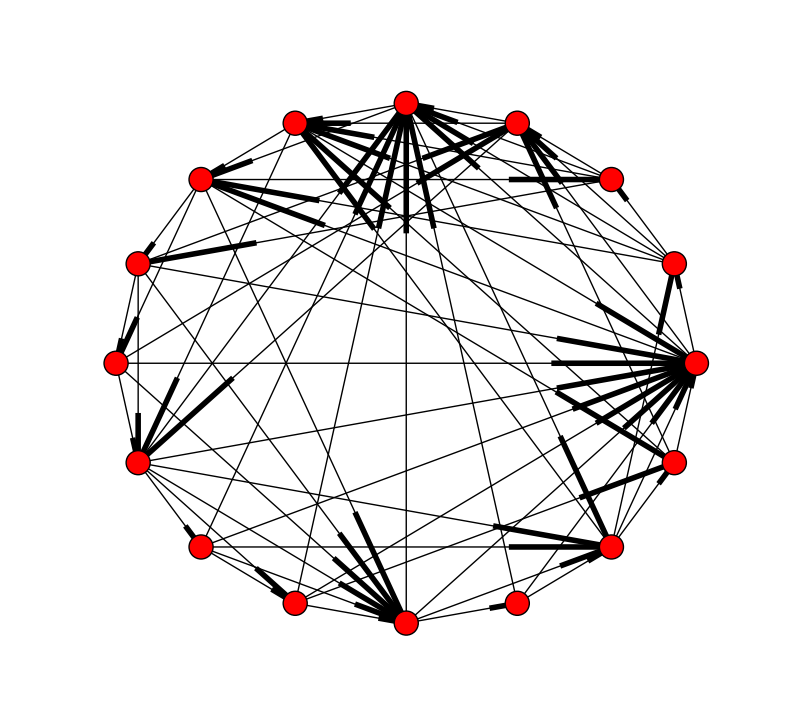
\includegraphics[width=\linewidth]{chordreal}
    \caption{A Chord ring with 16 nodes.  The bold lines are incoming edges.  Each node has a connection to its successor, as well as 4 fingers, some of which are duplicates.}
    \label{chordreal}
\end{figure}


With this scheme, we can reliably find the node responsible for some key by asking the next node in the circle for the information, who would then pass the request through the circle until the successor was found.  We can then proceed to directly connect with the successor to retrieve the file.  This naive approach is largely inefficient, and is a simplification of the lookup process, but it is the basis of how Chord theoretically works.

To speed up the lookup time, each node builds and maintains a \emph{finger table}.  The \emph{finger table} contains the locations of up to $m$ other nodes in the ring (Figure \ref{chordreal}).  The $i$th entry of node $n$'s \emph{finger table} corresponds to the node that is the $successor(n+2^{i-1})$ $mod$ $2^m$. Hash values are not perfectly distributed, it is possible to have duplicate entries in the \emph{finger table}. 


\begin{figure}
    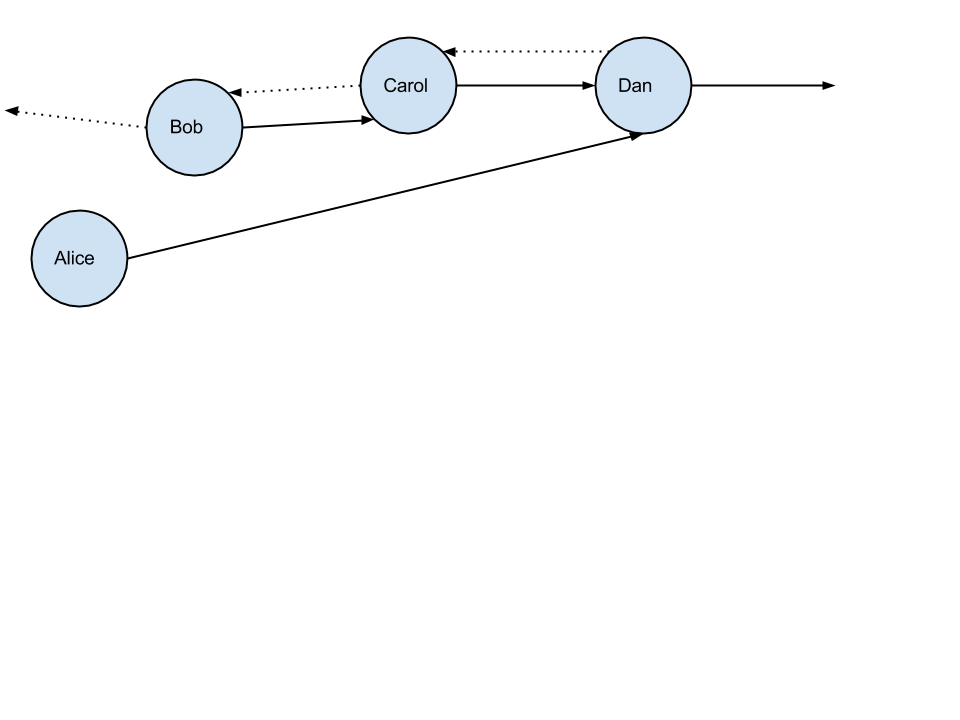
\includegraphics[width=\linewidth]{abcd1}
    \caption{Alice has incorrectly determined that Carol is her appropriate successor.  When Alice stabilizes, Carol will let her know about Bob.}
    \label{abcd1}
\end{figure}


\begin{figure}
    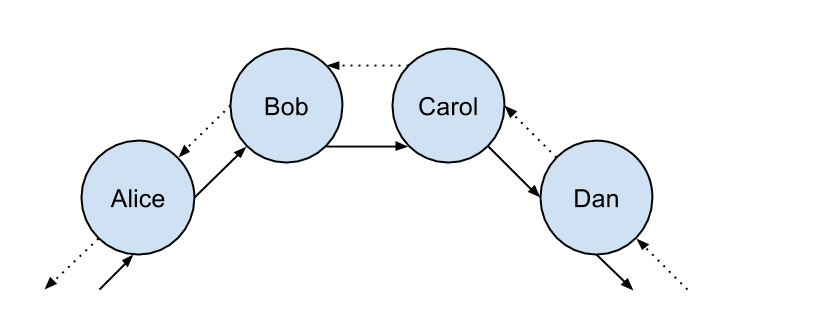
\includegraphics[width=\linewidth]{abcd2}
    \caption{After completing stabilize, Alice makes Bob her successor and notifies him. Bob then made Alice as his predecessor.}
    \label{abcd2}
\end{figure}



When a node $n$ is told to find some key, $n$ looks to see if the key is between $n$ and $successor(n)$ and return $successor(n)$'s information to the requester. If not, it looks for the entry in the finger table for the closest preceding node $n'$ it knows and asks $n'$ to find the successor.  This allows each step to skip up to half the nodes in the network, giving a $\log_2(n)$ lookup time.  Because nodes can constantly join and leave the network, each entry in the table is periodically checked and updated. 

To join the network, node $n$ first asks $n'$ to find $successor(n)$ for it.  Node $n$ uses the information to set his successor, but the other nodes in the ring will not acknowledge $n$'s presence yet.  Node $n$ relies on the stabilize routine to fully integrate into the ring.

The stabilize routine helps the network integrate new nodes and route around nodes who have left the network. Each node periodically checks to see who their successor's predecessor is.  In the case of a static network, this would be the checking node.  However, if the checking node gets back a different node, it looks at that returned node's hash value and changes their successor if needed.  Regardless of whether the checking node changes its successor, that node then notifies the (possibly) new successor,  who then checks if he needs to change his predecessor based on this new information.  While complex, the stabilization process is no more expensive than a heartbeat function.  A more concrete example:


Suppose Alice, Bob, Carol, and Dan are members of the ring and everyone happens to be ordered alphabetically (Figure \ref{abcd1}). Alice is quite sure that Carol is her successor.  Alice asks Carol who her predecessor is and Carol says Bob is.  Since Bob is closer than Carol, Alice changes her successor to Bob and notifies him.  

When Bob sees that notification, he can see Alice is closer than whoever his previous predecessor is and sets Alice to be his predecessor.  During the next stabilization cycle, Alice will see that she is still Bob's predecessor and notify him that she's still there (Figure \ref{abcd2}).



%\subsection{Extensions of Chord}

%The Cooperative File System (CFS) is an anonymous, distributed file sharing system built on top of Chord \cite{CFS}.  In CFS, rather than storing an entire file at a single node, the file is split up into multiple chunks around 10 kilbytes in size.  These chunks are each assigned a hash and stored in nodes corresponding to their hash in the same way that whole files are.  The node that would normally store the whole file instead stores a \emph{key block}, which holds the hash address of the chunks of the file. 

%The chunking allows for numerous advantages.  First, it promotes load balancing. Each piece of the overall file would (ideally) be stored in a different node, each with a different backup or backups.  This would prevent any single node from becoming overwhelmed from fulfilling multiple requests for a large file.  It would also prevent retrieval from being bottlenecked by a node with a relatively low bandwidth. Finally, when Chord uses some sort of caching scheme like that described in CFS \cite{CFS}, caching chunks as opposed to the entire file resulted in about 1000 times less storage overhead.  

%Mutable files  and  IRM, which is short for Integrated File Replication and Consistancy Maintenence, has nodes keep track of file requests they initiate or forward.  If they find they are frequently forwarding a request for a particular file, they store that file locally until it is no longer requested frequently.  What makes IRM unqiue is that it combines caching with a 

%Chunking also opens up the options for implementing additional redundancy such as erasure codes \cite{rizzo1997effective}. With erasure codes, redundant chunks are created but any combination of a particular number of chunks is sufficient to recreate the file.  For example, a file that would normally be split into 10 chunks might be split into 15 encoded chunks.  The retreival of any 10 of those 15 chunks is enough to recreate the file.  Implementing erasure codes would presumably make the network more fault tolerant, but that is an exercise left for future work.


%Generally, related files should be kept together; Chord, however, just hashes the filename to find the responsible node and sends it to that location without any thought to organization.  Our solution to this is to use allow the file owner to select first 80 bits of a file's hash, then generating the remaining least signifcant bits by hashing the filename.  It does not matter if a file owner, in some infintesimally small coincidence, chooses the same 80 bit prefix as another file owner, as the purpose is to keep related files together.   



\subsection{MapReduce and Hadoop}
At its core, MapReduce \cite{mapreduce} is a system for division of labor, providing a layer of speration between the programmer and the more complicated parts of parallel processing.  The programmer sends a large task to a master node, who then divides that task among slave nodes (which may further divide the task).  This task has two distinct parts: Map and Reduce.  Map performs some operation on a set of data and then produces a result for each map operation.  This intermediate data can then be reduced, combining these sets of intermediate data into a set, which is further combined with other sets.  This process continues until one set of data remains.

The classic example given for MapReduce is counting the occurrence of each word in a collection of documents.  The master node splits up the documents into multiple chunks and sends them off to workers.  Each worker then goes through each chunk and creates a small word frequency list.  These lists are then used by other workers, who combine them into larger and larger lists, until the master node is left with a word frequency list of all the words in the documents. 



%The most popular platform for MapReduce is Hadoop \cite{Hadoop}. Hadoop is an open-source Java implementation deveolped by Apache and Yahoo! \cite{pavlo2009comparison}.  Hadoop has two components, the Hadoop Distributed File System (HDFS) and the Hadoop MapReduce Framework \cite{mrsurvey}.  Under HFDS, nodes are arranged in a heirarchical tree, with a master node, called the NameNode, at the top.  The NameNode is responsible for keeping track of which DataNodes posess which files as well as other metadata essential for controlling the netowork. MOVE THIS DOWN
 

One very popular open-source implementation of MapReduce is Apache's Hadoop \cite{Hadoop}.  Hadoop serves as both a distributed file system and framework for MapReduce \cite{shvachko2010hadoop}.  However,  Hadoop's MapReduce framework is very strongly tied to the Hadoop Distributed File System (HDFS) and the hierarchy of servers that is used by it.  Hadoop is centralized around the NameNode.  The NameNode's job is to organize and distribute information to the slave nodes, called DataNodes.  This makes the NameNode a single point of failure \cite{shvachko2010hadoop} in the network, as well as a potential bottleneck for the system \cite{hadoop-bottle}.

To do work on Hadoop, the user stores thier data on the network.  This is handled by the NameNode, which equally apportions the data among the DataNodes.  When a user wants to run some analysis on the data or some subset the data, then that function is sent by the NameNode to each of the DataNodes that is responsible for the indicated data.   After the DataNode finishes processing, the result is sent handled by yet another node called a Reducer.

Key differences between Hadoop and ChordReduce are discussed in Section V.


\section{Related Work}

We have identified two extant that focus on combining P2P concepts with MapReduce.  Both papers are similar to our research, but differ in crucial ways.

\subsection{P2P-MapReduce}
Marozzo et al. \cite{marozzo2012p2p} investigated the issue of fault tolerance in centralized MapReduce architectures such as Hadoop.  They focused on creating a new, P2P based MapReduce architecture called P2P-MapReduce.  P2P-MapReduce is designed to be more robust at handling node and job failures during execution.

Rather than use a single master node, P2P-MapReduce employs multiple master nodes, each responsible for some job.  If one of those master nodes fails, another will be ready as a backup to take its place and manage the slave nodes assigned to that job.  This avoids the single point of failure that Hadoop is vulnerable to. Failures of the slave nodes are handled by the master node responsible for it.

Experimental results were gathered via simulation. Their results showed that while P2P-MapReduce generated an order of magnitude more messages than a centralized approach, the difference rapidly began to shrink at higher rates of churn.  However, when looking at actual amounts of \emph{data} being passed around the network, rather than the number of messages, the bandwidth required by the centralized approach greatly increases as a function of churn, while the distributed approach again remains relatively static in terms of increased bandwidth usage and messages sent.  

They concluded that P2P-MapReduce would, in general, use more network resources than a centralized approach. However, this was an acceptable cost as the P2P-MapReduce would lose less time from node and job failures \cite{marozzo2012p2p}.

Our work differs from Marozzo et al.'s in that P2P-MapReduce does not examine leverage using the underlying strengths of a particular P2P protocol or group of protocols, which would have made the architecture simpler.  P2P-Mapreduce is decentralized, but still relies on a very definite master/slave hierarchy, while all nodes in ChordReduce are both workers and masters.  We also implemented our MapReduce system rather than simulating the work.

\subsection{MapReduce using Symphony}

ADDRESS FAULT TOLERANCE
Lee et al.'s work more strongly resembles our own in that their system uses a P2P protocol to perform Map Reduce \cite{leemap}.  Their work, like ours, draws attention to the fact that a P2P network can be much more than a way to distribute files and demonstrates how to accomplish different tasks using map and reduce functions.

Rather than using Chord, Lee et al. used very similar DHT protocol with a ring topology, Symphony \cite{symphony}\footnote{I can expand here on Symphony if we need space, but I think that is better suited for the journal paper}.  To run a MapReduce job over the Symphony ring, a node is selected by the user to effectively act as the master.  This ad-hoc master then performs a bounded broadcast over a subsection the ring.  Each node repeats this broadcasts over a subsection of that subsection, resulting in a tree with the first node at the top.  Map tasks are disseminated evenly throughout the tree and their intermediate results are reduced on the way back up to the ad-hoc master node.  This allows the ring to disseminate Map and Reduce tasks without the need for a coordinator responsible for distributing these tasks and keeping track of them, unlike Hadoop.
 

Their deployed experimental results showed that the latency experienced by a centralized configuration is similar to the latency experienced in a completely distributed framework.

One of the major improvements that can be made to Lee et al.'s method is improving the fault tolerance of the system.  While in most cases the network is able to cope with churn via the underlying Symphony protocol, no arrangements are made to handle the loss of nodes during the execution of a MapReduce task \cite{leemap}.  This means the MapReduce operation on Symphony has the same single point of failure Hadoop has. 

ChordReduce exploits the backup feature used for files to protect MapReduce tasks from failure.  Our network can handle the failure of the node our reduced data is being sent to, as the data is being sent to a address on the ring, rather than a particular node.


%\subsubsection{Underlying protocol: Chord vs Symphony}

%\cite{leemap}is implemented on top of BruNet\cite{BruNet}, which itself is an implantation of the DHT protocol Symphony \cite{symphony}.  Symphony and Chord share a great deal of symetry.  Both protocol create an overlay in the shape of a ring, both  use a hash to assign files to a node that corresponds to that hash, and both use a finger table\footnote{For simplicity, we use the Chord terminology in discussing Symphony concepts. The \emph{long-distance links} are analogous to Chord's fingers and the \emph{short-distance links} correspond to the predecessor and successors of a node.} to create shortcuts across the ring.

%The difference is that Symphony seeks to exploit the small world phenomena \cite{kleinberg2000navigation}, where the fingers are chosen at random along a probability distribution function.  The further away a node is, the less likely it will be chosen as a finger \footnote{Check this with brendan.}.  Like Chord, messages travel along the paths that bring them closest to their target destination, which is the node responsible the destination's hash value.  In a network with  $N$ nodes, each with $k$ fingers, a message will take on average $O(\frac{1}{k} \log^{2}(N))$ hops to reach its destination.   In comparison, the average lookup time in Chord is $\frac{1}{2}\log(N)$ \cite{Chord}.

%To speed up routing in Symphony, the fingers are bidirectional, rather than unidirectional (does this mean when k is 4 there's effectively 8 fingers?  I think it does according to the \# tcp connection).  Symphony also has nodes maintain a 1-lookahead list for each finger \footnote{these speedups could be implemented on chord.}.

%In the simulation of a $2^15$ node network in \cite{symphony}, this allowed the Symphony to perform at nearly identical speeds with Chord while utilizing only 4 bidirectional fingers and a 1-lookahead.  With 27 bidriectional finger and 1-lookahead, Symphony's lookups took half the time that Chord did. 

%However, for large numbers of fingers, keeping a lookahead list becomes expensive.   Unless their metrics for Symphony are actually log base 10, then it's unbelievable amazing looking.  I have my doubts there.


%\subsection{Volunteer Computing}
%In recent years, there has been a trend of crowd-sourcing large and complicated tasks among willing participants.  Folding@home is a distributed program for simulating the way proteins put themselves together, a process called folding \cite{folding}.  \cite{folding}.  The program has been a huge boon to the research of various diseases, such as Alzheimer's Disease, cystic fibrosis, and Huntington's Disease.  These diseases and others are believed to be tied to proteins misfolding, or failing to assemble properly.  Folding@home simulates the molecular dynamics of proteins during the folding process, with the aim to understand  how misfolds occur\footnote{Get this entire paragraph reviewed by a bio guy}.  A fast processor can simulate about 20 nanoseconds of behavior a day, but protein interactions occur at the millisecond and second scale, which necessitated a distributed approach.  

%This concerted effort has been immensely successful, providing data for 109 peer-reviewed publications as of August 2013 \cite{foldingPapers}\footnote{Check the format of this citation}.

%In a similar vein, SETI@home is a concerted effort by millions of users to analyze collected radio signals for signs of intelligent life \cite{anderson2002seti}\footnote{Check the sizes, I think seti is bigger}.

%Great Internet Mersenne Prime Search, or GIMPS, is a large scale distributed computing software to find Mersenne Primes.  Mersenne primes are prime numbers of format $M_{p} = 2^{p} - 1$, where $p$ is a prime number. The largest known prime number is a Mersenne Prime found using GIMPS.

%Our program would provide an excellent platform for users to write their own program for volunteer work.  
%\subsection{P2P-MapReduce Systems}

\section{ChordReduce}


%ChordReduce does not use the bounded broadcast approach presented by Lee et al., but it would not be difficult to implement it through Chord.  ChordReduce instead randomly chooses a hash address to receive a particular map operation, ensuring that such tasks are evenly distributed accross the network.
\subsection{Motivation}



Marozzo et al. \cite{marozzo2012p2p} shows that adding additional fault-tolerance features to a MapReduce architecture is worth the added cost of maintenance, as the time lost due to node failures is greatly reduced.  However, Marozzo et al. do not explore the benefits of leveraging the properties of a P2P protocol to reduce the complexity of the architecture and completely distribute the responsibility of the task across the network.  As a result, P2P-MapReduce still relies on specific nodes to coordinate the network's actions.

Lee et al.'s \cite{leemap} explores the benefits of building a MapReduce module to run on top of an existing P2P protocol, specifically Symphony.  This allows the MapReduce tasks to be executed without the need of a central source of coordination, unlike Hadoop.  The MapReduce architecture is constructed at runtime, via bounded broadcast. Despite these benefits, the Symphony based MapReduce architecture would be greatly improved by the addition of components to handle the failure of nodes during execution.  As it stands now, if a node crashes the job will fail due to the loss data

Both these papers have promising results and confirm the capability of our own framework.  ChordReduce uses Chord to act as a completely distributed topology for MapReduce, negating the need to assign any explicit roles to nodes or have a scheduler or coordinator.  ChordReduce does not need to assign specific nodes the task of backing up work; nodes backup their tasks using the same process that would be used for any other data being sent around the ring.  Finally intermediate data works its way back to a specified hash address, rather than a specific hash node, eliminating any single point of failure in the network.  The result is a simple, distributed, and highly robust architecture for MapReduce.


\subsection{Chord Implementation of Handling node failures.}
When a node $n$ changes his successor, $n$ asks if the successor is holding any data $n$ should be responsible for.  The successor looks at all the data $n$ is responsible for and sends it  to $n$.  The successor does not have to delete this data. If fact, keeping this data as a backup is beneficial to the network as a whole, as $n$ could decide to leave the network at any point. 

Due to the potentially volatile nature of a peer-to-peer network, Chord has to be able to handle (or at the very least, tolerate) an arbitrary amount of churn.  Section II described how Chord gradually guides nodes into their correct locations after they join the network.  The same is true for when a node leaves the network; the stabilize procedure will guide nodes to their correct successors and predecessors.  However, we can exert more control over how to handle nodes leaving the network

Chord specifies two ways a node can leave the ring.  A node can either suddenly drop out of existence, or a node can tell the network he is about to leave, letting his successor and predecessor immediately perform the needed changes.

When a node politely quits, he informs both his successor and predecessor and gives them all the information they need to fill the gap that would be left over. He also sends all of the data he is responsible for to his successor, who would become responsible for that data when that node left.  Fingers that pointed to that node would be corrected during the finger maintenence period.  This allows for the network to adjust to the change with a minimum of fuss.

Unfortunately, it is impossible that every time a node leave the network it will do so politely.  If a node suddenly quits, the data it had stored goes with it. To prevent data from becoming irretrievable, a node can periodically send backups to its successor.  So as not to overwhelm the ring with a cascade of backups of backups, the node only passes along what it considers itself responsible for, which changes as nodes enter and leave the network.  If the backup leaves, he send his stuff to his successor, since the backup's successor would be the one responsible for the info now. 

Our prototype framework does not implement a polite disconnect;  when a node quits, it does so quickly and abruptly.  This design forced us to ensure that system would be able to handle churn under the worst of cases.  Polite quit could be implemented quite easily, but it would provide minimal benefit for our use cases. 


\subsection{Implementation Details}

ChordReduce, at its core, is a fully functional Chord implementation in Python.  Our installation was designed to be as simple as possible.   It consists of downloading our code \cite{code} and running chord.py.  You can specify a port and IP and port of a node in the ring you want to join.  With this minimal information, the node will automatically integrate into the ring.

Other than a hashing library, we wrote the protocol and networking code from scratch.  Once we could create a stable ring, we created various services to run on top the network, such as a file system.  Our file system is capable of storing whole files or splitting the file up among the ring. Our MapReduce module is a service that runs on top of our Chord implementation, just like our file service.    We avoided any complicated additions to the Chord architecture; instead we used the protocol's properties to create the features we desired in our MapReduce framework. 
  
In our implementation of MapReduce, each node takes on responsibilities of both a worker and master, much in the same way that a node in a P2P file-sharing service will act as both a client and a server.  To start a job, the user contacts a node a specified hash address and provides him with the tasks and data. 

The job of this stager is to take the work and divide it into \emph{data atoms}, which are the smallest individual units that work can be done on.  This might be a line of text in a document, the result of a summation for a particular intermediate value, or a subset of items to be sorted.  The specifics of how to divide the work are defined by the user in a \emph{stage} function.  These data atoms are then given a random hash and sent to that hash address, guaranteeing an even distribution of the data atoms throughout the network.  The data atoms also contain the Map function and Reduce function, as defined by the user.  A job ID is also included, so that data atoms from different jobs can be differentiated.

Nodes which receive data atoms apply the map function to the data to create intermediate data atoms, which are then sent back to the stager's hash address (or some other user defined address).  Traveling using Chord's fingers, this will take $\log n$ hops.  At each hop, the node waits a predetermined minimal amount of time to accumulate additional intermediate data atoms (In our experiments, this was .1 seconds).%\footnote{Actual footnote: The amount of time spent waiting can be manipulated to tradeoff between time spent reducing and network usage}.  

Nodes that receive at least two intermediate data atoms merge them into one data atom using the Reduce function.   The atoms are continually merged until only one remains at the hash address of the stager. 

Once the reductions are finished, the user retreives his results from the node at the stager's address.  This may not be be the stager himself, as once the stager has sent all the data atoms, his job is done.  The stager does not need to collect the results himself, since the work is sent to the stager's hash address, rather than the stager itself.  Thus, the stager could quit the network after staging, and both the user and the network would be unaffected by the change. % Here, we are leverging two features. First, we use the automatic assignment of responsibility to automatically route the data to the sucessor.  %Second, the same process Chord uses to backup files is used to backup the intermediate data. 

Similar precautions are taken for nodes working on Map and Reduce tasks.  Those tasks get backed up by a node's successor, who will run the task if the node quits the network before the doing the job (e.g. the successor loses his predecessor).   The task is given a timeout by the node.  If the backup node detects that the responsible node has failed, he starts work and rebacks up to his successor.  Otherwise, the data is tossed away once the data expires. This is done to prevent a job being submitted twice if $n$ goes down after finishing his task and sending it out.

An advantage of our system is the ease of development and deployment.  The developer does not need to worry about distributing work evenly, nor does he have to worry about any node in the network going down.  The underlying Chord ring handles that automatically.  If a node joins the ring as the MapReduce process is running, that node can be assigned work automatically.  The stager does not need to keep track of the status of the network.  In a node goes down while performing an operation, his successor takes over for him.  If the user finds they need additonal processing power during runtime, they can boot up additional nodes, which would automatically be assigned work based on their hash value.  This makes the system extremely robust during runtime.

All a developer needs to do is write three functions: the staging function, Map, and Reduce.  These define how to split up the work into manageable portions, the work to be performed on each portion to get some results, and how to combine these results into a single result, respectively. 

While MapReduce is most efficient when each node is physically close in a cluster, minimizing the impact of latency, this does not exclude the option of tasks being distributed throughout the world.  This setup may be more applicable to a volunteer computing framework, such as Folding@home \cite{folding}.

Many clusters assume identical or near identical hardware, running an equal amount of nodes, performing an equal amount of work. This is not always a safe assumption to make.  If the hardware used for computations is not equal, then some processors can be left idling when they could be doing more work, while others may be overwhelmed, holding back the rest of the network.

Adjustments can be easily made on the user's end.  If some hardware can take more work than others, then that system can boot up more instances of nodes locally. Running two nodes locally would mean that approximately twice as much work would assigned to that computer.  Automatically balancing this load is an avenue for future research.


%\subsubsection{Just Chord or can we use a different Protocol}
%This architecture can be adapted for any P2P protocol that has features similar to Chord: consistant hashing, automatic routing and responsiblilty handling.


\subsection{Comparison of ChordReduce and Hadoop}

The centralized structure of Hadoop requires that the NameNode be solely responsible for keeping track of where all the data is in the network \cite{Hadoop}.  ChordReduce has two options for the handling the data used for performing MapReduce.  Data may be distributed by the stager along with the dissemination of the Map and Reduce functions.  The data may also be stored in the ring \cite{CFS}.  In either case, no single node is responsible for knowing the location of all of the data.  

The knowledge of the locations of the files in ChordReduce is distributed among the entire network and requires an intelligent procedure to send and store large volumes of data.  Attempting to distribute each data atom via its own individual message would overwhelm the networking library. Thus, when the stager distributes data atoms, it sends at most one message to each of its fingers.  This message contains the subset of data atoms for which that subsection of the network is responsible for.  This data is further divided by those servers such that the data atoms are distributed via an emergenent minimum spanning tree, similar to the bounded broadcast used in \cite{leemap}.  The intermediate data being sent back using the Chord routing protocol produces a similar emergent tree. 

The execution of the Reduce stage in this manner prevents the node responsible for the final result from being overwhelmed with traffic \cite{hadoop-bottle}.  This configuration ensures that the average amount of data transfered between any two nodes is less than or equal to $\frac{size of all intermediate data}{number of nodes}$.  This assumes that the Reduce step results in a data atom whose contents are equal to or less than the size of the combined intermediate data.  


\section{Experiments}
In order for ChordReduce to be a viable framework, we had to show that:
\begin{enumerate}
    \item it could provide a significant speedup when a job was distributed
    \item ChordReduce scales
    \item ChordReduce handles churn during execution
\end{enumerate}
Speedup first can be demonstrated by showing that, in general, a distributed job performs quicker than the same job handled by a single worker.  To establish scalability, we need to show that the overhead of distributing the work grows logarithmically with the number of workers.  In addition, we need to demonstrate that the larger the job is, the number of nodes we can have working on the problem, without the overhead incurring diminishing returns, increases. Finally to demonstrate robustess, we need to show that ChordReduce can handle arbitrary node failure in the ring and that such failures minimally impact overall speedup of the network.


More formally we need establish that $\exists n$ such that $T_{n} < T_{1}$, where $T_{n}$ is the amount of time it takes for $n$ nodes to finish the job.  In addition, to establish scalability,

$$T_{n} = \frac{T_{1}}{n} + k \cdot \log_{2}(n)$$, where $\frac{T_{1}}{n}$ is the amount of time the job would take when distributed in an ideal universe and $k \cdot \log_{2}(n)$ is network induced overhead, $k$ being an unknown constant.

%In an ideal universe, where the movement of data from one node to another is instantanous, scalabilty would not be an issue.  A job with five nodes working on it would be 5 times faster than a job be executed by a single node.  In other words, $T_{n} = \frac{T_{1}}{n}$, where $T_{n}$ is the amount of time it takes for $n$ nodes to finish the job.  However, distributing the job across multiple nodes incurs a .  To establish scalability, we need to show that there is some $p$ workers  
%The goal of these experiments is to prove that speedup behavior follows the approximate equations 
%
%$$T_{n} = \frac{T_{1}}{n} + k \cdot \log_{2}(n)$$
%$$speedup = \frac{T_{1}}{\frac{time_{solo}}{n} + k \cdot \log_{2}(n)}$$ 
%where $n$ is the number of nodes in the network, $time_{solo}$ is the amount of time a job would take without parallelization, and $k \cdot \log_{2}(n)$ is network induced overhead. $k \cdot \log_{2}(n)$  is a measure of additional time spent on the problem due to network latency and maintenence and grows logarithmically proportion to $n$.  It reflects that for each problem, there is a point at which that the cost of parallization starts providing dimishing returns.  $k$ is unique to each problem.

\subsection{Setup}
\begin{figure}
    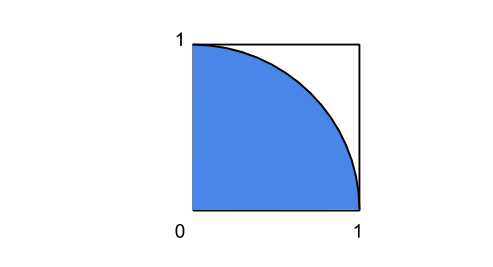
\includegraphics[width=\linewidth]{dartboard}
    \caption{The "dartboard." The computer throws a dart by choosing a random $x$ and $y$.  If $x^{2} + y^{2} < 1^{2} $, the dart landed inside the circle.}
    \label{dartboard}
\end{figure}


To stress test our framework, we ran a Monte-Carlo approximation of $\pi$. This process is largely analogous to having a square with the top-right quarter of a circle going through it (fig. \ref{dartboard}), and then throwing darts at random locations. Counting the ratio of darts that land inside the circle to the total number of throws give us an approximation of $\frac{\pi}{4}$.  The more darts thrown, i.e. the more samples that are taken, the more accurate the approximation\footnote{This is not intended to be a particularly good approximate of $\pi$. Each digit of accuracy requires increasing the number of samples taken by an order of magnitude.}.

We chose this experiment for a number of reasons. The job is extremely easy to distribute. Each map job is defined by the number of throws the node needs to make and yields an intermediate result containing the number of throws that the node made and the number of throws that landed inside the circular section.  Reducing intermediate results is then a matter of adding the respective fields together. 

This also made it very easy to test scalability. By doubling the amount of samples, we can double the amount of work each node gets.  We could test also test the effectiveness of distributing job among different numbers of workers. 

We ran our experiments using Amazons's EC2 service.  Each node was an individual EC2 small instance \cite{amazon-instances} with a preconfigured Ubuntu 12.04 image.  These instances were capable enough that they could provide constant computation, but still weak enough that they would be overwhelmed by traffic on occasions, creating a constant churn effect in the ring.  

Once started, nodes pull the latest version of the code and run it as a service, automatically joining the network.  We can choose any arbitrary node as the stager and tell it to run the MapReduce process. We found that the network was robust enough that we could take a node we wanted to be the stager out of the network, modify its MapReduce test code, have it rejoin the network, and then run the code new code without any problems. Since only the stager has to know how to create the map tasks, the other nodes don't have to be updated and are happy to perform the tasks they are given.

Our experiments were ran on groups of 1, 10, 20, 30, and 40 nodes.  Each sized ring was asked to generate $10^{9}$ samples by default, with later tests done on $10^{8}$ and $10^{10}$.  Due to the size of the $10^{8}$ job, we also gathered data for 5 nodes. 

We also had at our disposal a subroutine called $plot$, which sends a message to sequentially around the ring to establish how many members there are.  If $plot$ failed to return in under a second, then the ring was undergoing some kind of instability.

\subsection{Results}

\begin{figure}
    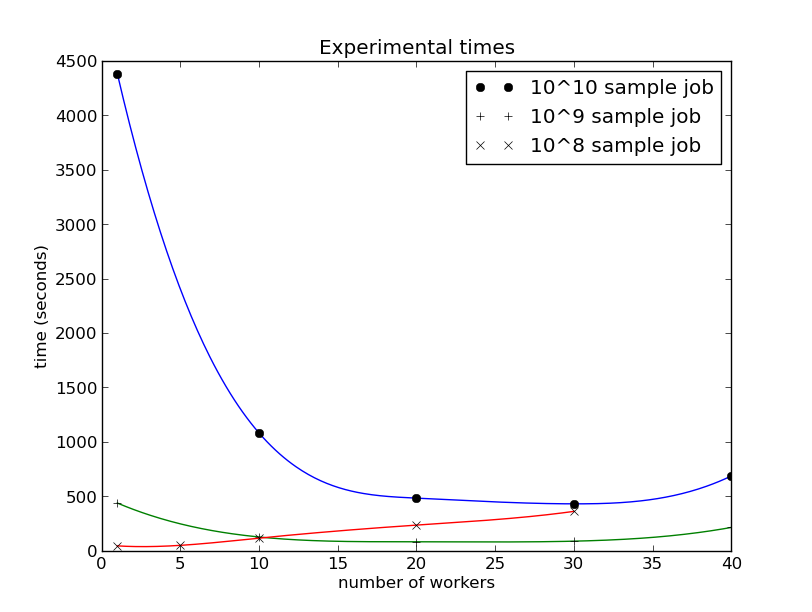
\includegraphics[width=\linewidth]{expTime}
    \caption{For a sufficiently large job, it was almost always preferable to parallelize it.  When the job is too small, such as with the $10^{9}$ data set, our runtime is dominated by the overhead.  Our results are what we would expect when overhead grows logarithmically to the number of workers}
    \label{expTime}
\end{figure}


\begin{figure}
    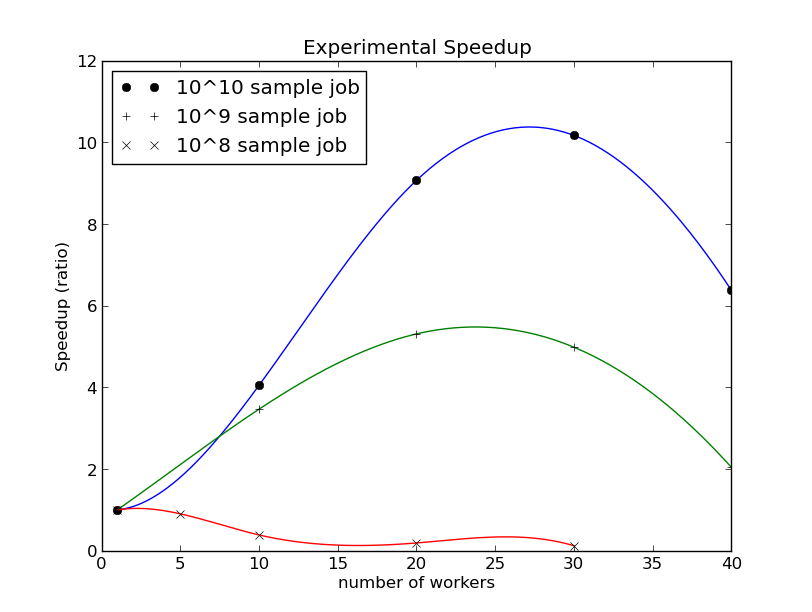
\includegraphics[width=\linewidth]{expSpeed}
    \caption{The larger the size of the job, the greater the gains of parallelizing with ChordReduce.  In addtion, the larger the job, the more workers can be added before we start seeing dimishing returns.  This demonstrates that ChordReduce is scalable.}
    \label{expSpeed}
\end{figure}

Our experiments show that for a given problem, ChordReduce can effectively parallelize the problem, yielding a substansial speedup.  Furthermore, our results showed that the larger the problem is, the more workers could be added before dimishing returns were incurred.  During run time, we experienced multiple instances where plot would fail to run and the stager would report socket errors, indicating that it had lost connection with a node in the ring.  Despite this turbulence, the nodes all managed to reestablish connection with each other and report back all the data.  This demonstrated that we were able to handle the churn in the network.

Our default series was the $10^{9}$ samples series.  On average, it took a single node 422 seconds, or approximately 7 minutes, to generate $10^{9}$ samples.  Generating the same number of points in parallel with 10, 20, 30, or 40 nodes was always quicker.  Notice that the samples were generated fastest when there were 20 workers, with a speedup factor of 4.83, while increasing the number of workers to 30 yielded a speedup of only 3.6.  At 30 nodes, the gains of parrellization were still there, but the cost of overhead ($k \cdot \log_{2}(n)$) had more of an impact.  This effect is more pronounced at 40 workers, with a speedup of 3.57.

Since our data showed that approximating $\pi$ on one node with $10^{9}$ samples took approximately 7 minutes, collecting $10^{10}$ samples on a single node would take 70 minutes at minimum.  Figure \ref{expSpeed} shows that the $10^{10}$ set gained greater benefit from parallization than the $10^{9}$ set.  Likewise, when compared to the $10^{9}$ set, more workers were able to participate before the ring began to experience diminishing returns.

The $10^{8}$ sample set confirms that the network overhead is logarithmic.  At that job size, the job is too small to be effectively parallelized and we start seeing overheard acting as the dominant factor in out dataset.  This matches the behavior predicted by our equation, $T_{n} = \frac{T_{1}}{n} + k \cdot \log_{2}(n)$. For a small $T_{1}$, $\frac{T_{1}}{n}$  approaches 0 as $n$ gets larger, while $k \cdot \log_{2}(n)$, our overhead, dominates the sample.  The samples from our dataset fit the curve $k \cdot \log_{2}(n)$, establishing that our overhead is increases logarithmicly with the number of workers.

%We discovered that some nodes having a high latency greately affects the value of $k$.

Since we have now established that $T_{n} = \frac{T_{1}}{n} + k \cdot \log_{2}(n)$, we can estimate how long a job that takes an arbitrary amount of time to run on a single node would take using ChordReduce.  Our data points indicated that the mean value of  $k$ was 36.5. The execution time is shown in Figure \ref{projTime} and the corresponding speedup in Figure \ref{projSpeed}.
Our data shows that the larger the job, the closer our speedup is to linear.  Figure \ref{projTime} shows that for jobs that would take more than $10^{4}$ seconds for single worker to complete, we can expect there would still be benefit to adding an additional worker, even when there are already 5000 workers already in the ring.  Figure \ref{projSpeed} further emphasizes this. Note that as the jobs become larger, the expected speedup from ChordReduce becomes closer and closer to linear.


\begin{figure}
    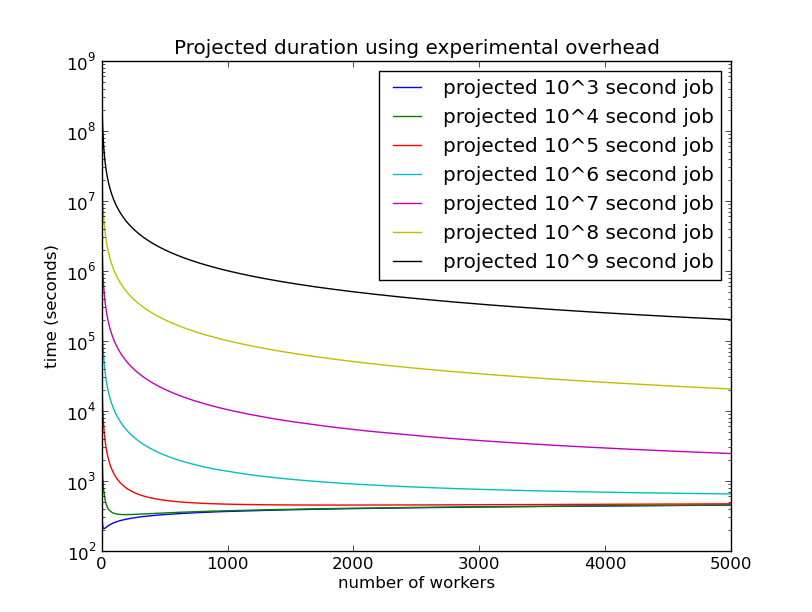
\includegraphics[width=\linewidth]{projTime}
    \caption{The projected runtime for different sized jobs using ChordReduce.  Each curve projects the behavior you would see if a job that takes a single worker the specified amount of time.}
    \label{projTime}
\end{figure}

\begin{figure}
    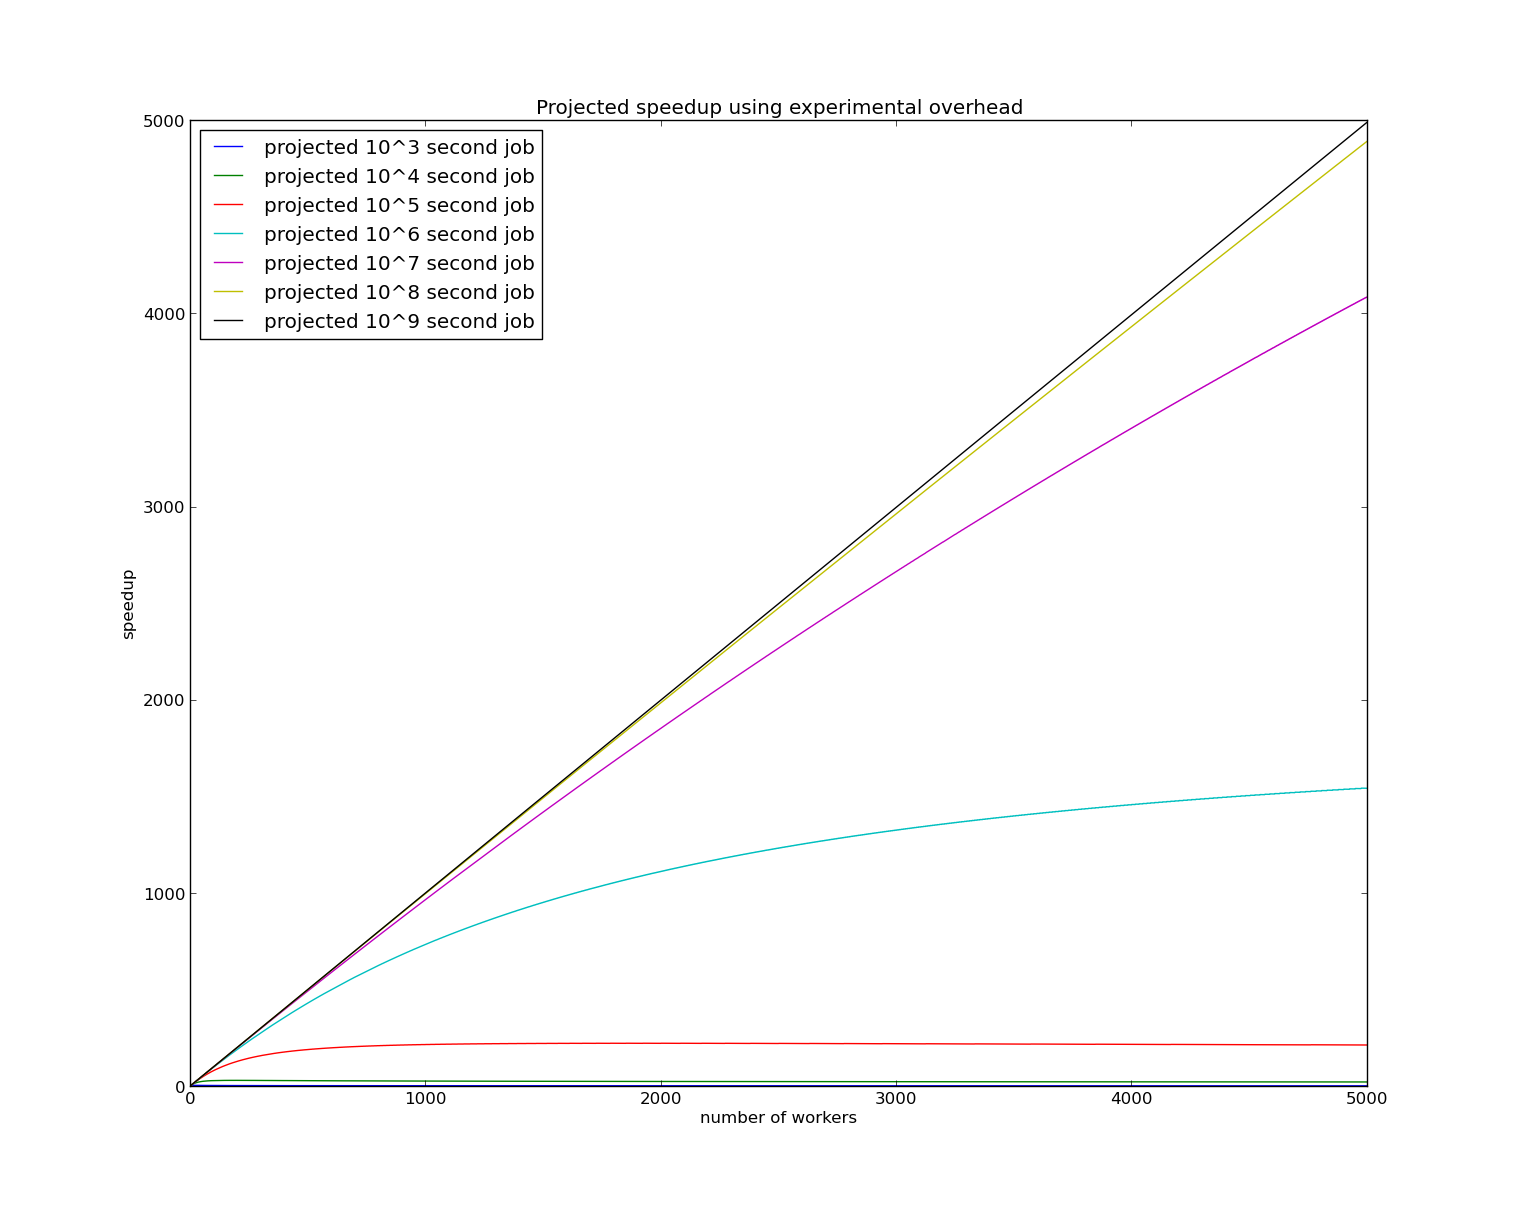
\includegraphics[width=\linewidth]{projSpeed}
    \caption{The projected speedup for different sized jobs. }
    \label{projSpeed}
\end{figure}


Figure CHURNSPEEDUP shows the experiments we ran for churn

\section{Conclusion and Future Work}
Chord, traditionally viewed as solely a P2P framework for distributing and sharing files, can be used as a platform for distributed computation.  Chord provides $\log(n)$ connectivity throughout 



So long as the average number of nodes in the ring remains the same, ChordReduce actually benefits from churn.
 
%ChordReduce is an effective platform because it scales logarithmically.  It is also able to handle churn during execution.
%However, MapReduce is not the only additional use for Chord.  Traditionally Chord is thought as a tool for P2P networks and file sharing.  We demonstrated through ChordReduce that Chord is much more than that.  Chord can serve as a scalable general purpose framework for distributed and cloud programming, thanks to its $\log(n)$ overhead.  We have identified many directions of future research for distributed programming using Chord.

Chord can would provide a suitable platform to solving problems that would otherwise be paticularally difficult, such as handling mutable data \cite{IRM}.  These same adjustments can be used to improve the latency of the Chord network, which was a major reason why a Chord-based distributed DNS \cite{cox2002serving} was abandoned.  

%Chord could also be used to create a distributed authentication service.

%Over the course of our development, we stumbled across various optimizations and tweaks that would be advantageous to Chord and our future research, but would have minimal impact on ChordReduce.  One of the major advantages of Chord is that all files are evenly distributed throughout the network.  However, there are some cases where it would be preferable to keep related files together.  We can do this by manually assigning the first $x$ bits of the $m$-bit length ID for the file, where $x \leq \frac{m}{2}$, then generating the remaining $m-x$ bits of the id with a hash function, as normal.  This would allow users to define a specific prefix for an abritrary group of files and keep them together on the network.


%Our future plans for ChordReduce itself is to recode the library in Java to take advantage of the multiprocessing support, which is limited in Python. 

TODO:
\begin{enumerate}
    \item Move specifics of our implementation over to ChordReduce
    \item Make sure all Map and Reduce are capitalized
    \item Define Job vs Task, make sure they are consistant
    \item Review networking terms with Dr. Anu
    \item Make sure out latex format for the title is what they want.
    \item Fix .bib Capitalizations
    \item Change parallelized  $\implies$ distributed
\end{enumerate}



\bibliographystyle{plain}
\bibliography{CHRONUS}
\end{document}

